\begin{figure}[t]
\centering
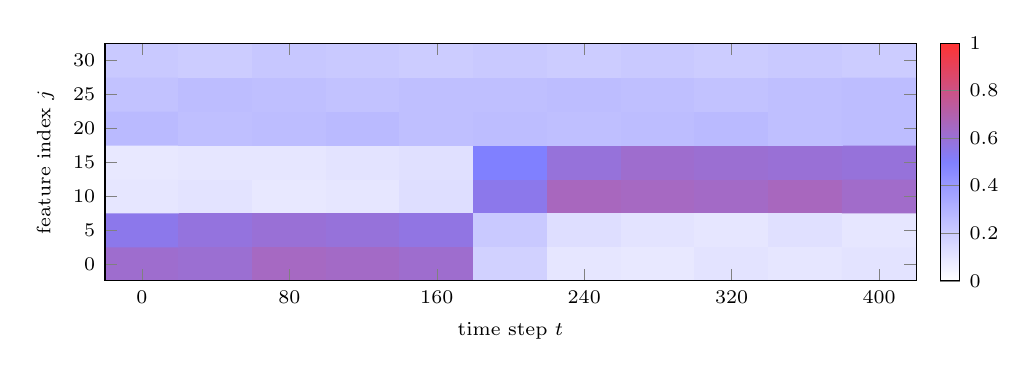
\begin{tikzpicture}
\begin{axis}[
    width=0.98\columnwidth,
    height=4.6cm,
    xlabel={time step $t$},
    ylabel={feature index $j$},
    enlargelimits=false,
    axis on top,
    colorbar,
    colormap={tafs}{color=(white) color=(blue!50) color=(red!80)},
    point meta min=0, point meta max=1,
    xtick={0,80,160,240,320,400},
    ytick={0,5,10,15,20,25,30},
    tick label style={font=\scriptsize},
    label style={font=\scriptsize},
    colorbar style={font=\scriptsize, width=0.25cm},
]
\addplot[
    matrix plot*,
    mesh/cols=11,
    point meta=explicit,
] table[meta=v] {
x y v
0 0 0.62
40 0 0.61
80 0 0.65
120 0 0.64
160 0 0.62
200 0 0.18
240 0 0.10
280 0 0.09
320 0 0.11
360 0 0.10
400 0 0.11
0 5 0.55
40 5 0.58
80 5 0.60
120 5 0.59
160 5 0.57
200 5 0.21
240 5 0.13
280 5 0.11
320 5 0.10
360 5 0.12
400 5 0.10
0 10 0.10
40 10 0.11
80 10 0.09
120 10 0.10
160 10 0.13
200 10 0.55
240 10 0.66
280 10 0.65
320 10 0.64
360 10 0.66
400 10 0.63
0 15 0.09
40 15 0.10
80 15 0.10
120 15 0.11
160 15 0.12
200 15 0.50
240 15 0.59
280 15 0.62
320 15 0.61
360 15 0.60
400 15 0.59
0 20 0.27
40 20 0.25
80 20 0.26
120 20 0.27
160 20 0.25
200 20 0.26
240 20 0.25
280 20 0.26
320 20 0.27
360 20 0.25
400 20 0.26
0 25 0.24
40 25 0.26
80 25 0.25
120 25 0.24
160 25 0.25
200 25 0.25
240 25 0.26
280 25 0.25
320 25 0.24
360 25 0.25
400 25 0.26
0 30 0.21
40 30 0.20
80 30 0.22
120 30 0.21
160 30 0.20
200 30 0.21
240 30 0.20
280 30 0.21
320 30 0.20
360 30 0.21
400 30 0.20
};
\end{axis}
\end{tikzpicture}
\caption{Per-step attention map averaged across heads on the synthetic regime-switch task. Each row is one of $p{=}32$ engineered features (top: lag/rolling; middle: exogenous; bottom: nuisance). The boundary at $t{=}200$ is clearly visible.}
\label{fig:attn_heatmap}
\end{figure}
